\subsection{Control PID acoplado}
El modelo que se ha venido trabajando posee la particularidad de que posee una unica entrada
y multiples salidas, es decir, es un modelo de tipo SIMO, esto complica un poco la
controlabilidad del sistema (usando la literatura clasica), pues un controlador PID estandar,
solo funciona para sistemas con la misma cantidad de entradas y salidas, como se explico
anteriormentelo que se suele hacer en la literatura es realizar la retroalimentacion sobre
un subconjunto de las variables tales que cumplan la condicion anterior.
El controlador que se presenta acontinuacion fue diseñado con el fin de resolver este
problema.
\subsubsection{Funcionamiento del control}
El controlador es fundamentalmente una suma de controles PID diferentes controladores,
cada uno de estos controladores recibe como señal de entrada la salida de la respectiva
variable que se desea controlar, para despues alimentar el sistema con la suma de estos.
Formalmente el control puede ser definido de la siguiente manera:
\begin{align*}
  u(t) =& K_{pc}e_c(t) + K_{ic}\int_0^te_c(t')dt' + K_{dc}\dfrac{de_{c}(t)}{dt} + \\
   & K_{pa}e_a(t) + K_{ia}\int_0^te_a(t')dt' + K_{da}\dfrac{de_{a}(t)}{dt}  
\end{align*}

donde $u(t)$ es la accion del controlador, $K_{pc}, K_{ic}, K_{dc}$, son las respectivas
contantes del controlador para el carrito y de manera simiar $K_{pa}, K_{ia}, K_{da}$,
son las constantes del controlador asociadas a la dinmaica del angulo; Y $e_c, e_a$ son
respectivamente los errores asociados a la posicion del carrito y al angulo.
El diagrama de bloques implementado puede verse en la~\ref{fig:controlS}

\begin{figure}[t]
  \label{fig:controlS}
  \includegraphics[scale=1]{Figuras/control-modelo.jpg}
  \caption{Diagrama de bloques de la implementacion del control PID acoplado} 
\end{figure}

\subsubsection{Estimacion de parametros}
Al momento de diseñar el controlador la parte mas complicada era precisamente encontrar los
valores optimos para las constantes $K_i$, esto se debe principalmente a el acoplamiento que
presentan ambos sistemas, pues aunque los controladores se encuentren independientes, ambos
realimentan el mismo sistema, haciendo que los cambios de una variable de estado
inminentemente afectaran la otra, esto, junto al desconocimiento del efecto que posee cada
parametro sobre el sistema, hace poco factible una sintonizacion manual u una sintonizacion
basada en metodos estandares. Es por esto que se optó por plantearla estimacion de parametros
como un problema de optimizacion no linel, que busca disminuir el error del estado
estacionario.
Para resolver este problema de optimizacion se utilizó un metodo metaheuristico, el metodo
GRASP el cual es ampliamente aplicado para resolver problemas de optimizacion combinatoria.
\subsubsection{GRASP}
El metodo GRASP fue introducido inicialmente por~\citet{Feo1989}, con el fin de solucionar
heuristicamente el problema del conjunto cobertura, un importante problema NP-completo,
sin embargo, con el tiempo el algoritmo fue adaptado para resolver diferentes problemas.
El algoritmo parte de una solucion inicial (en nuestro caso un conjunto de constantes $K_i$
aleatorias, e iterativamente realiza modificaciones sobre dicha soluciones, esto se realiza
alternando las diferentes constantes de manera independinte a la misma solucion y luego se
evalua cada uno de los nuevos conjuntos de parametros en la funcion objetivo; En un algoritmo
voraz clasico se escogería como la siguiente solucion, el mejor movimiento, que mejore la solucion
anterior, sin embargo esta manera de proceder puede caer muy facilmente en un optimo local, el metodo
GRASP plantea una manera diferente de proceder, este considera las $n$ mejores soluciones y de estas
considera una aleatoria, esto aumenta la diversidad en las soluciones y hace mas complicado caer en
en optimo local.\\
La mejor solucion encontrada por el metodo fue
\[K = \]

y la respuesta al impulso puede verse en la figura~\ref{fig:control}
\begin{figure}[t]
  \label{fig:controlS}
  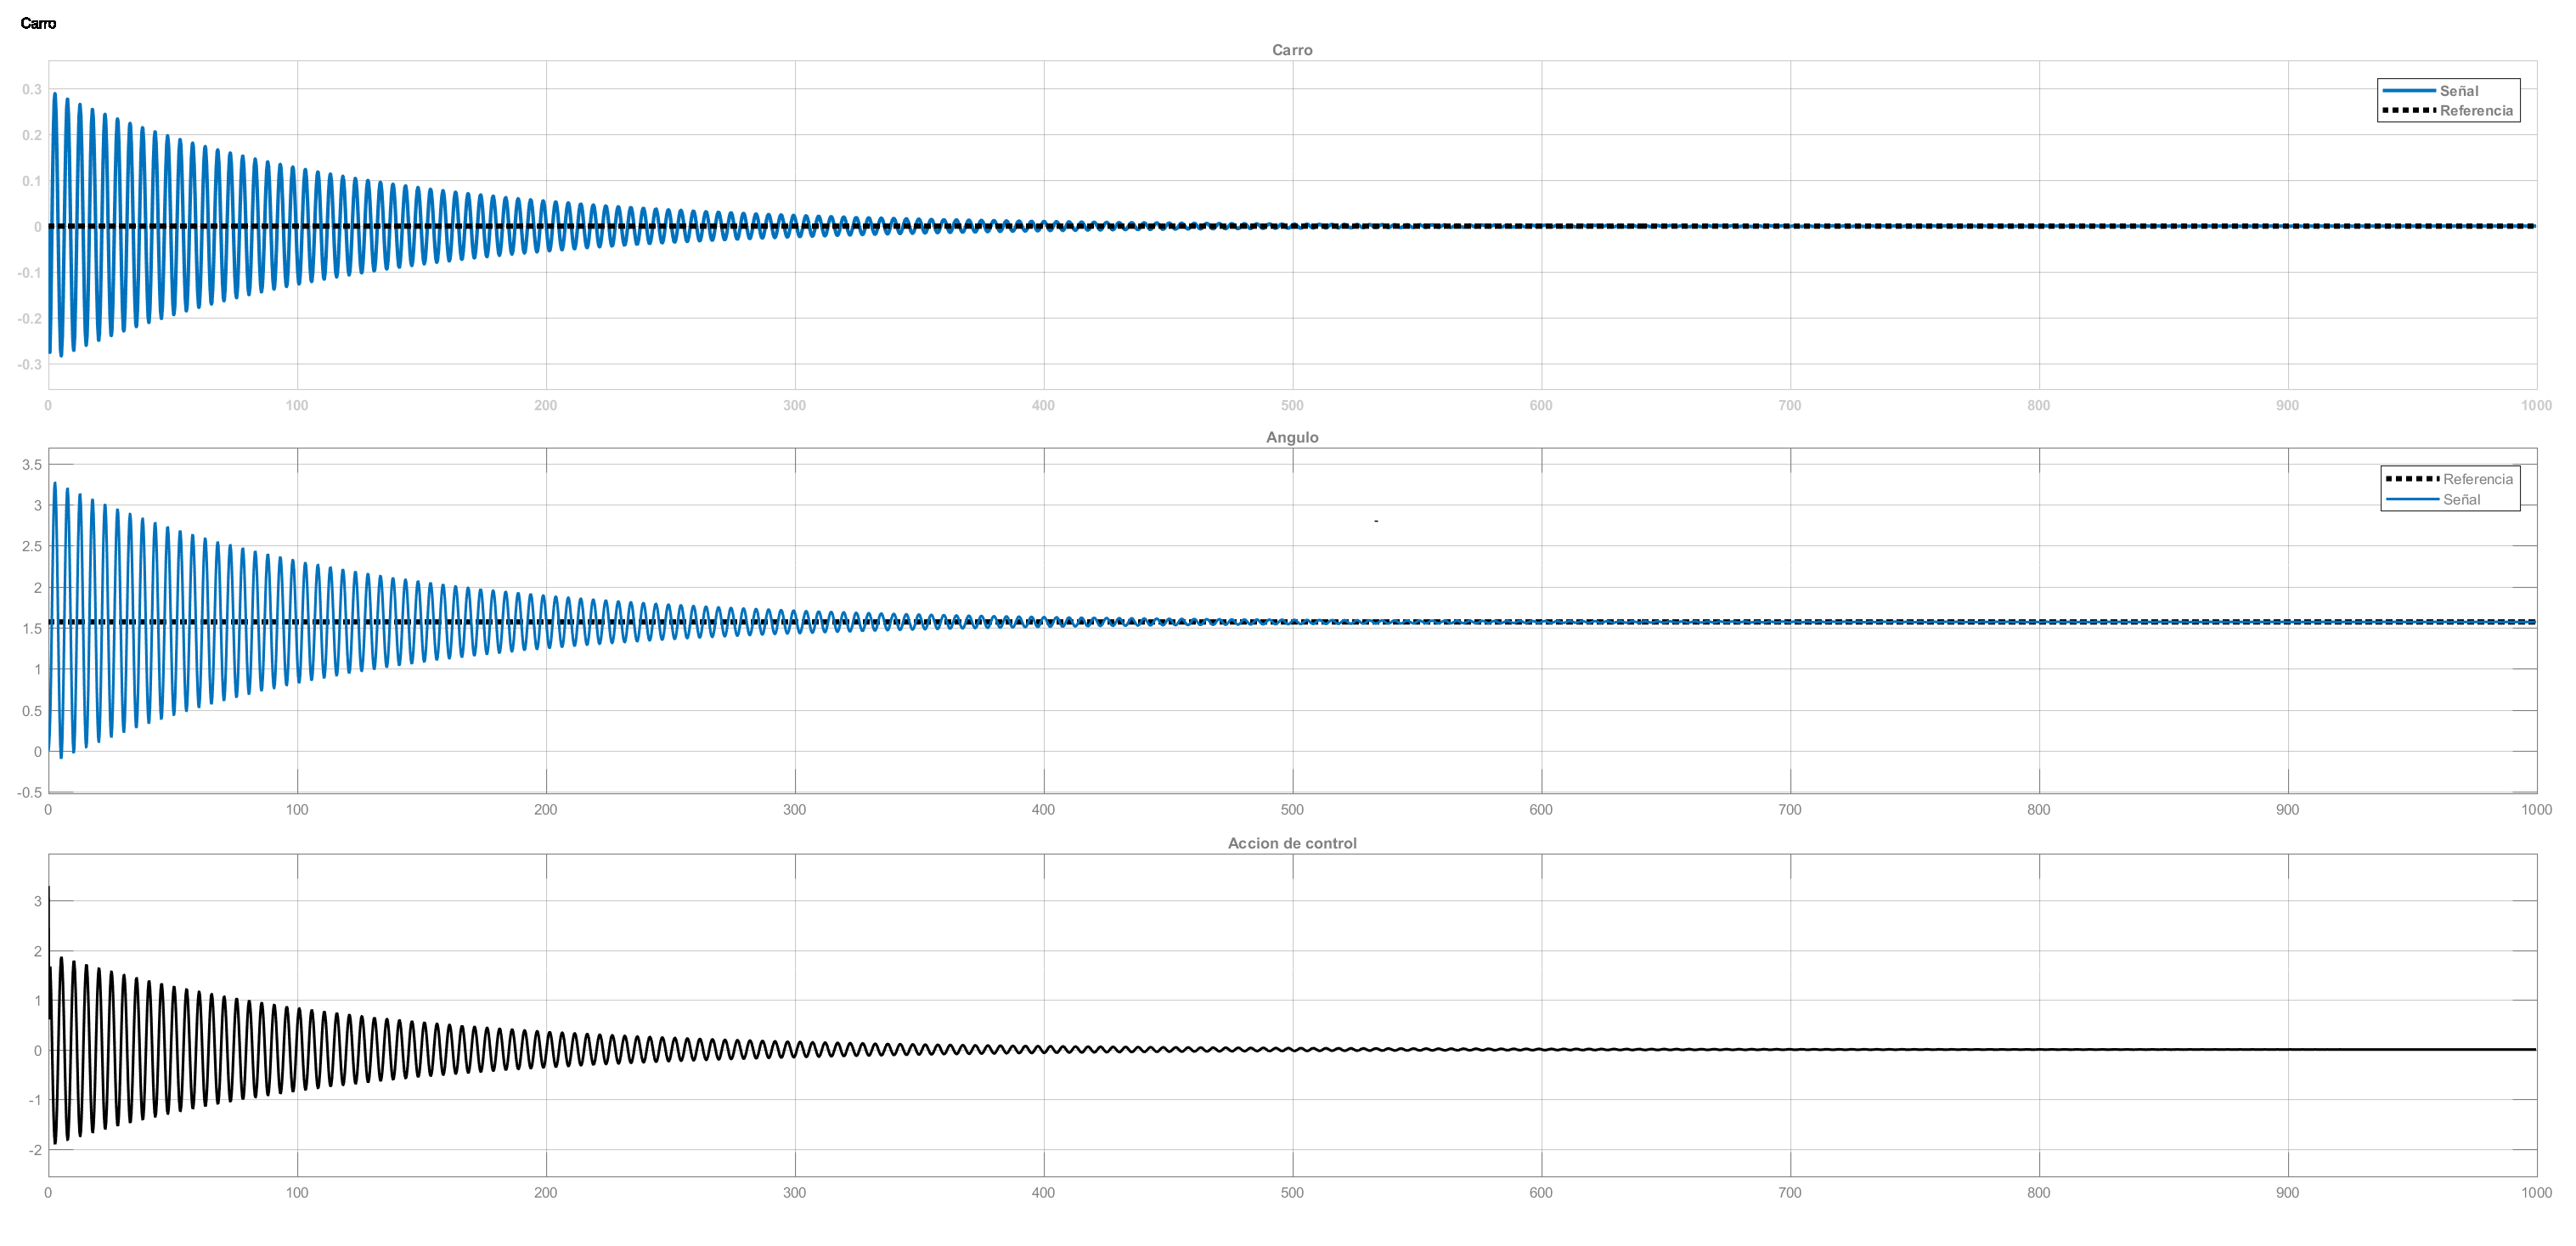
\includegraphics[scale=1]{Figuras/controlS}
  \caption{Diagrama de bloques de la implementacion del control PID acoplado} 
\end{figure}

De la respuesta anterior, se puede ver que el control es capaz de controlar apropiadamente ambas
señales a su señal de referencia, lo cual puede llegar a ser una gran ventaja en comparacion
a lo controladores presentados anteriormente. Adicionalmente al plantear la sincronizacion del
controlador como un problema de optimizacion, es posible resolverlo con diferentes metodos, tales
como algoritmos geneticos, los cuales en principio permitirían tener un control inteligente.